\documentclass[uplatex,12pt]{jsarticle}
\usepackage[dvipdfmx]{graphicx}
\usepackage{url}
\usepackage{listings,jlisting}
\usepackage{ascmac}
\usepackage{amsmath,amssymb}

%ここからソースコードの表示に関する設定
\lstset{
%  basicstyle={\ttfamily},
  basicstyle={\small},
  identifierstyle={\small},
%  commentstyle={\smallitshape},
%  commentstyle={\small\itshape},
  commentstyle={\small\ttfamily},
  keywordstyle={\small\bfseries},
  ndkeywordstyle={\small},
  stringstyle={\small\ttfamily},
  frame={tb},
  breaklines=true,
  columns=[l]{fullflexible},
  numbers=left,
  xrightmargin=0zw,
  xleftmargin=3zw,
  numberstyle={\scriptsize},
  stepnumber=1,
  numbersep=1zw,
  lineskip=-0.5ex
}
%ここまでソースコードの表示に関する設定

\title{知能プログラミング演習II 課題2}
\author{グループ8\\
  29114060 後藤 拓也\\
}
\date{2019年10月28日}

\begin{document}
\maketitle

\paragraph{提出物} rep3

\paragraph{グループ} グループ8

\paragraph{グループメンバー}
\begin{center}
\begin{tabular}{|c|c|c|}
  \hline
  学生番号&氏名&貢献度比率\\
  \hline\hline
  29114003&青山周平&no\\
  \hline
  29114060&後藤拓也&no\\
  \hline
  29114116&増田大輝&no\\
  \hline
  29114142&湯浅範子&no\\
  \hline
  29119016&小中祐希&no\\
  \hline
\end{tabular}
\end{center}
\paragraph{自分の役割} 必須課題3.3
\\ 「知識システムの質問応答システム」
%%%%%%%%%%%%%%%%%%%%%%%%%%%%%%%%%%%%%%%%%%%%%%%%%%%%%%%%%%%%%%%%%%%%%%%%%%%%%%
\section{課題の説明}
\begin{screen}
課題3-1または3-2で作った知識表現を用いた質問応答システムを作成せよ.
なお,ユーザの質問は英語や日本語のような自然言語が望ましいが,難しければ課題2で扱ったような変数を含むパターン (クエリー) でも構わない.
\end{screen}

\section{手法}

\begin{enumerate}
\item 課題2で扱ったような変数を含むクエリーによる質問
\item 英文による質問
\end{enumerate}

\subsection{手法1に関して}
変数(?xや?yなど)を含み, [Tail, Label, Head]の形を守って代入する. 具体的には「Taro hobby baseball」という英文ではなく, 単なるクエリーに対して, 「Taro hobby ?x」といったクエリーの形に添った質問をするといった手法である.

\subsection{手法2に関して}
ある一定の知識システムが構築された状態において, 質問する内容というのは自ずと限られてくる. 今回は質問とそれに基づく応答を大きく以下の2パターンに分けている. 

\begin{enumerate}
\item 疑問詞Whatに基づく質問から,  ?xの内容を答える
\item 質問の内容に対して, YesかNoかで答える
\end{enumerate}

1. の疑問詞を含む質問に関しては, 質問の内容からどのようにHead, Tail, Labelを取り出すかは, 以下の図1を参照してほしい.
\begin{figure}[htbp]
 \begin{center}
  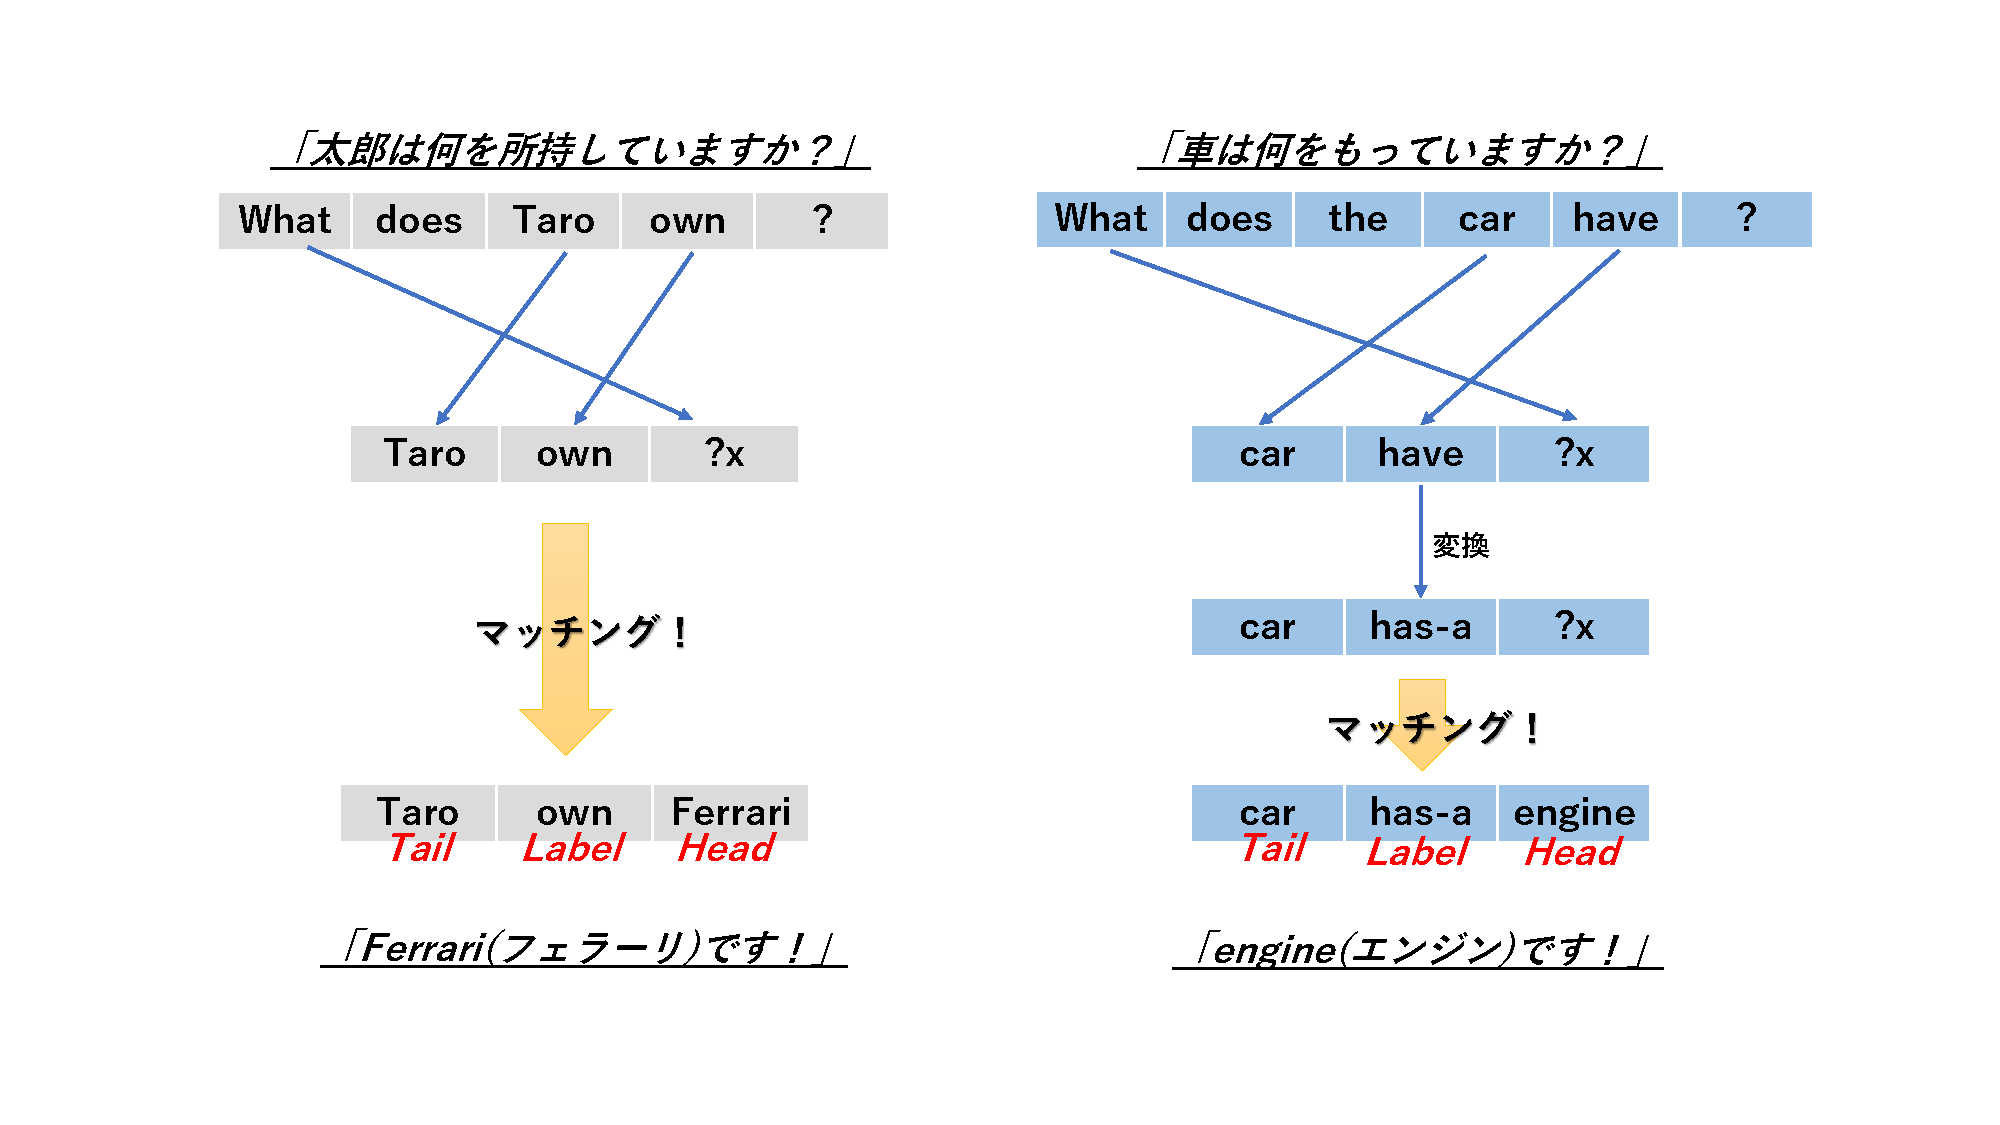
\includegraphics[width = 9cm, pagebox = cropbox, clip]{英文構造_疑問詞SVO.pdf}
 \end{center}
 \caption[]{SVO構造による疑問詞の質問}\label{fig:fig1.1}
\end{figure}

英語の第3文型SVO型は, S(主語)がTail, V(動詞)がLavel, 0(目的語)がHeadになっている. その形に沿って, 疑問文から要素を抽出する. もちろん, 前置詞の処理や, haveをhas-a関係に合わせるなどの調整も必要である.

この質問は"Whatを使って問われる内容は, 目的語の部分のみ"というのを暗示している. 「車はエンジンを持つ」という1文が存在する際に, 「車は何を持ちますか?」とは聞けても, 「エンジンを持っているのは何ですか」とは聞けない. \\

2. のYesかNoで答える質問に関しても, 以下の図2のように分解できる.
\begin{figure}[htbp]
 \begin{center}
  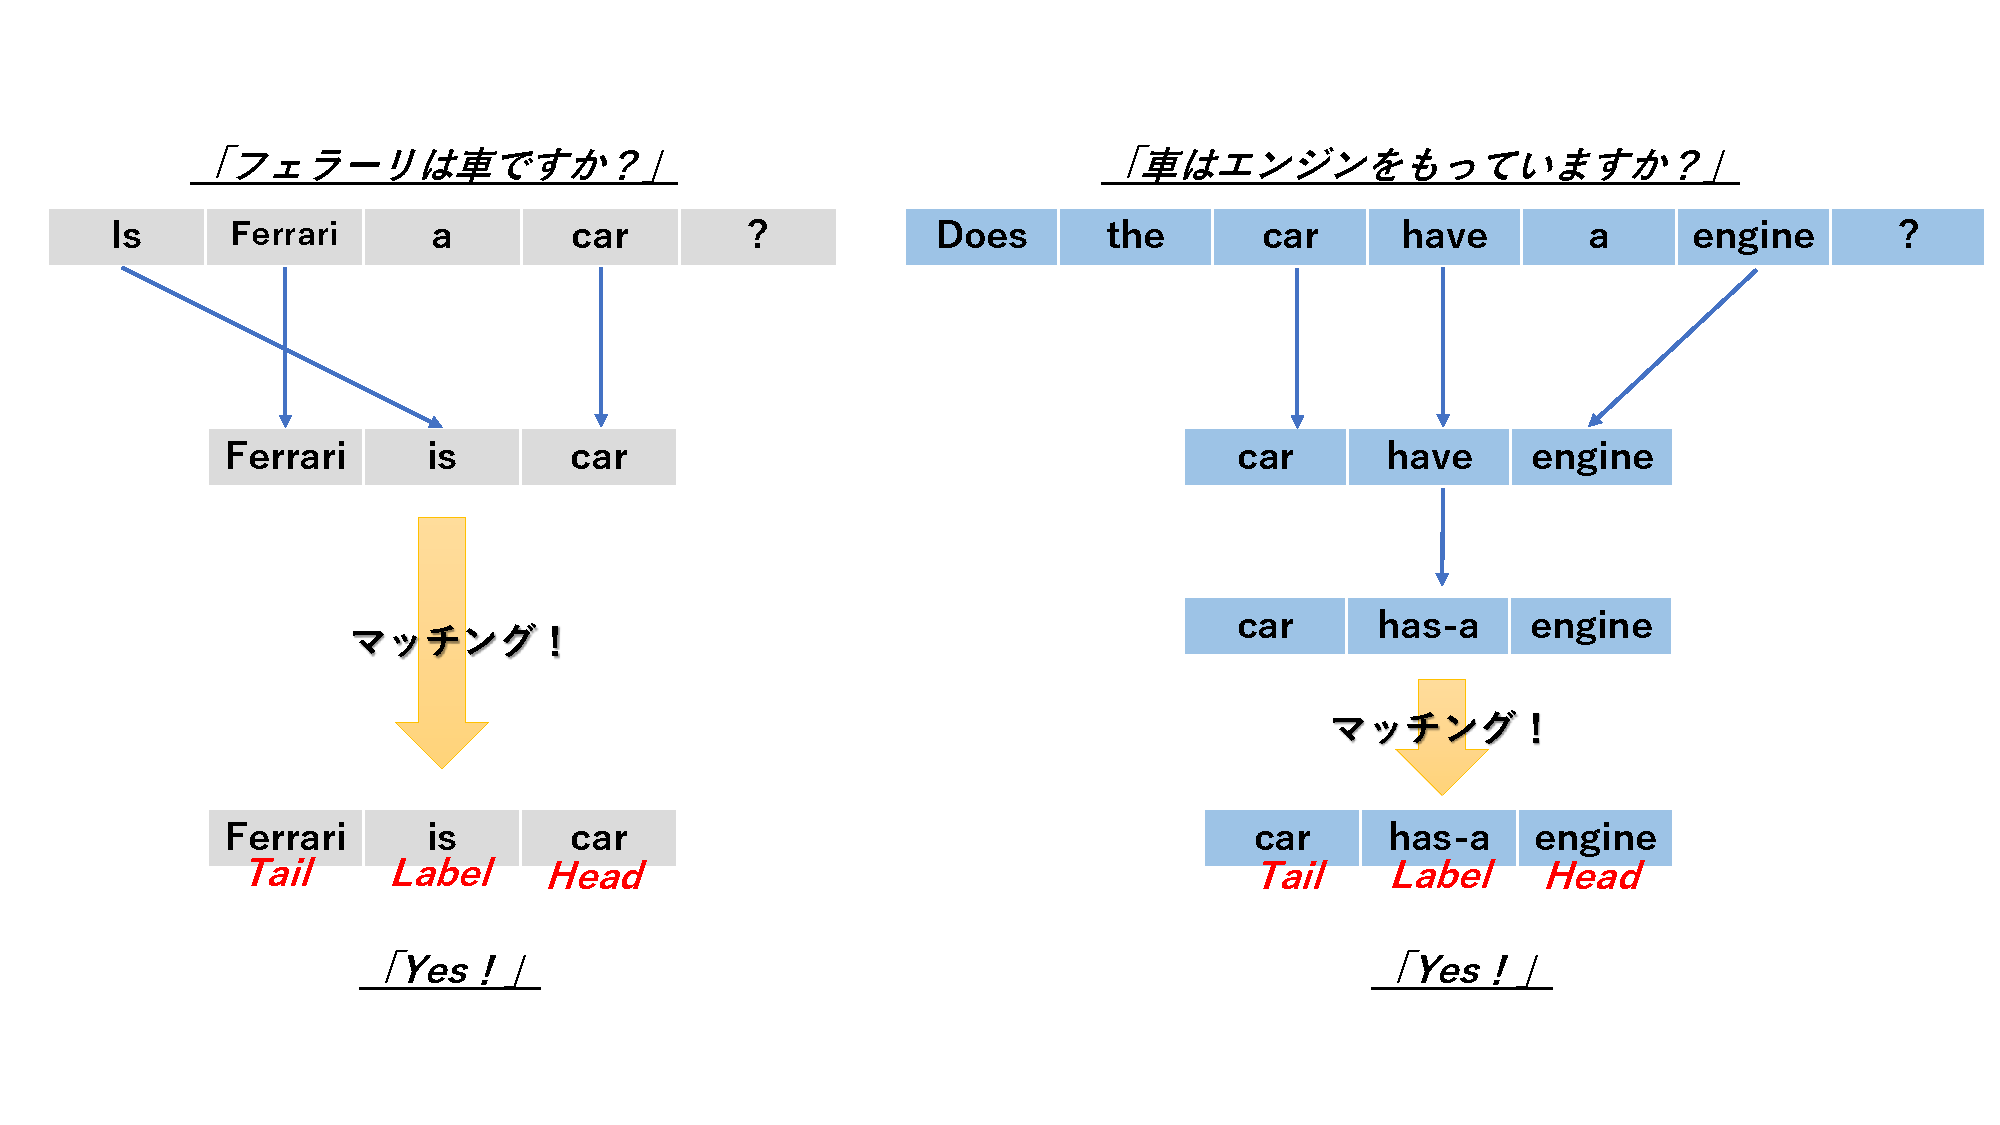
\includegraphics[width = 9cm, pagebox = cropbox, clip]{英文構造_YesNo型.pdf}
 \end{center}
 \caption[]{Yes/Noで答える型}\label{fig:fig1.1}
\end{figure}

 同様にSVCをそれぞれTail, Lavel, Headに合わせ, マッチングが成功したら, 「Yes」を返し, 失敗した場合は「No」を返す.

そして, だれもが違和感を覚えたのは, 「Taro hobby baseball」という1文. 何となく「太郎の趣味は野球です」になるが, Google翻訳にかけたら, 「ヒロキホビーサッカー」である. そもそもhobbyは動詞になり得ない. 正しくは, 「Taro's hobby is baseball」である. これに質問をするには, 「Is Taro's hobby a baseball ?」に対応する必要がある. そのため, 図2のようなLabelの取り方ではいけない. 質問において, 2つ目のトークンに「's」があるかどうかで処理を変える.

\section{実装}
\subsection{手法1}
まずは, 手法1に関する「課題2で扱ったおうな変数を含むクエリーによる質問」の部分を実装したソースコード\ref{src:No1}に示す。
\begin{lstlisting}[caption=クエリーの形に添った質問応答, label=src:No1]
/***
 * 課題2で扱ったような変数を含むパターン (クエリー)による質問応答システム
 * "?x is-a sports"と"?y hobby ?x"をとらえる
 * → 質問は3つのトークンに分けられる
 */
Scanner stdIn1 = new Scanner(System.in);	//文字列読み込み
Scanner stdIn2 = new Scanner(System.in);	//数値読み込み
ArrayList<ArrayList<String>> queryList 
    = new ArrayList<ArrayList<String>>(); //質問(query)を入れる
StringTokenizer st;		//トークンごとに分解
int retry;
do {
	ArrayList<String> tokenList = new ArrayList<>();
	System.out.println("質問を入力してください");
	String s = stdIn1.nextLine(); 	//質問文がここに入り,
	st = new StringTokenizer(s);	//トークンごとに分解し,
	for(int i=0; i<st.countTokens(); i++) {
		tokenList.add(st.nextToken());
	}
	tokenList.add(st.nextToken());
	queryList.add(tokenList);
	System.out.println("もう1つ? 1...Yes/ 0...No");
	retry = stdIn2.nextInt();
}while(retry == 1);

ArrayList<Link> query = new ArrayList<Link>();
for(int i=0; i<queryList.size(); i++) {
	query.add(new Link(queryList.get(i).get(1), queryList.get(i).get(0), queryList.get(i).get(2)));
}
sn.query(query);
\end{lstlisting}

上記のプログラムはmain文において, 全てのリンクをSemanticNetクラスのインスタンスに加えて後で行われ, その後, queryメソッドを呼び出している. 質問文はJavaの文字列読み込みのScannerクラスを用いている. それにより入力されたString型のデータを空欄があるたびに分割するStringTokenizerを利用して各トークンに分け, それぞれを適切にTail, Label, Headに分け, queryメソッドを呼び出している.\\

\subsection{手法2}
次に, 「英語の質問応答システム」の条件分岐の部分をソースコード\ref{src:No2}に示す.
\begin{lstlisting}[caption=英語における質問応答, label=src:No2]
	ArrayList<String> tokenList = new ArrayList<>();
	System.out.println("質問を入力してください");
	String s = stdIn1.nextLine(); 	//質問文がここに入り,
	st = new StringTokenizer(s);	//トークンごとに分解し,

	String firstToken = st.nextToken();
	String secondToken = st.nextToken();
	if(firstToken.equals("What")) {
		if(secondToken.equals("does")) {
			String thirdToken = st.nextToken();
			if(thirdToken.equals("the")) 
				thirdToken = st.nextToken();
			tokenList.add(thirdToken);
	
			String forthToken = st.nextToken();
			if(forthToken.equals("have"))
				tokenList.add("has-a");
			else
				tokenList.add(forthToken);
			tokenList.add("?x");
		}
	
		else if(secondToken.equals("is")) {
			String thirdToken = st.nextToken().replace("'s", "");
			tokenList.add(thirdToken);
			tokenList.add(st.nextToken());
			tokenList.add("?x");
		}
	}
	else if(firstToken.equals("Is")) {
		if(secondToken.contains("'s")) {
			tokenList.add(secondToken.replace("'s", ""));
					・
					・	   		//以下"Is"における"Yes, No返答"の
					・			//細かい条件分岐が行われている.

\end{lstlisting}

各トークンのメソッドを参照するnextTokenメソッドは呼び出すたびに, 次のトークンへ参照先が移ってしまうので, 条件分岐をする際には, firstToken, secondTokenのように一度String型に格納している. \ref{src:No2}の最初のif文では, 手法2で述べた1つ目の応答パターン「疑問詞Whatに基づく質問」の詳細と, 2つ目の応答パターン「Yes, Noで答える質問」の冒頭が示されている. 疑問詞Whatの後には, SVO関係の場合には"does"が, SVC構文の時には"is"とさらに2パターンに分かれている. 前置詞theを飛ばしたり, haveをhas-aに変更するなどを行う. 

ここでポイントになるのは, 質問文には必ず"(空欄) + ?"を入れてもらいたいということだ. というのも, nextTokenメソッドは呼び出し後に次のトークンを参照するので, もし"(空欄) + ?"がなければ, 文を最後まで参照した後に, 参照する次のトークンがなくなってしまい, エラーになってしまうからである.

\section{実行例}
\subsection{手法1}
日本語で言うと, [スポーツを趣味にしている人はだれか?]と質問したときの実行結果が以下のようになる.
\begin{lstlisting}
Successfully started
検索結果を取得
質問を入力してください
?x is-a sports
もう1つ? 1...Yes/ 0...No  1
質問を入力してください
?y hobby ?x
もう1つ? 1...Yes/ 0...No  0
*** Query ***
?x  =is-a=>  sports
?y  =hobby=>  ?x
[{?x=baseball, ?y=Taro}]
\end{lstlisting}

まずはスポーツが何か(?x)を求め, その後, そのスポーツに該当する何か(?y)を趣味としている人を探す. 正しい関係性が出力されていることが確認される.

ここで注目したいのは, 1回の実行における複数の質問内容は"かつ"の条件で結ばれているということである. これはソースコード\ref{src:No1}をみるとわかることだが, do-whileでループさせることで, queryメソッドに入れる内容が増え, SemanticNetクラスのqueryLinkメソッドで, 新しいリンクが構築されていくからである.

\subsection{手法2}
\begin{lstlisting}
質問を入力してください
What is Taro's speciality ?
*** Query ***
Taro  =speciality=>  ?x
{?x=AI}です.
もう1回? 1...Yes/ 0...No 1
質問を入力してください
Is Taro a NIT-student ?
*** Query ***
Taro  =is-a=>  NIT-student
Yes!
もう1回? 1...Yes/ 0...No 1
質問を入力してください
Is Taro a student ?
*** Query ***
Taro  =is-a=>  student
Yes!
\end{lstlisting}

適切な英語で質問をすることで, 結果が返ってくる. Goole翻訳を使うことをお勧めする. 上記の例では, 「太郎はNITの生徒」と「生徒は勉強しない」から「太郎は勉強しない」がうまく結果として出力されていることがわかる.

また, 手法1とは異なり, "かつの関係"をもって複数の質問をする機能はつけていない. 入力した1つ質問に対して, 1つの答えが出力される. 

\section{考察}
次の質問とそれの回答を見てほしい.
\begin{lstlisting}
*** Query ***
Taro  =own=>  ?x
{?x=Ferrari}です.
もう1回? 1...Yes/ 0...No 1
質問を入力してください
Is Ferrari a car ?
*** Query ***
Ferrari  =is-a=>  car
Yes!
もう1回? 1...Yes/ 0...No 1
質問を入力してください
Does Taro own car ?
*** Query ***
Taro  =own=>  car
No...
\end{lstlisting}

文章的には, 「太郎はフェラーリを持っていて, フェラーリは車なのだから, 太郎は車をもっている」と思うが, このプログラムの継承の仕方ではうまくいかない. 継承にはLabel名が関わっているのである. 以下の図を見てもらいたい.
\begin{figure}[htbp]
 \begin{center}
  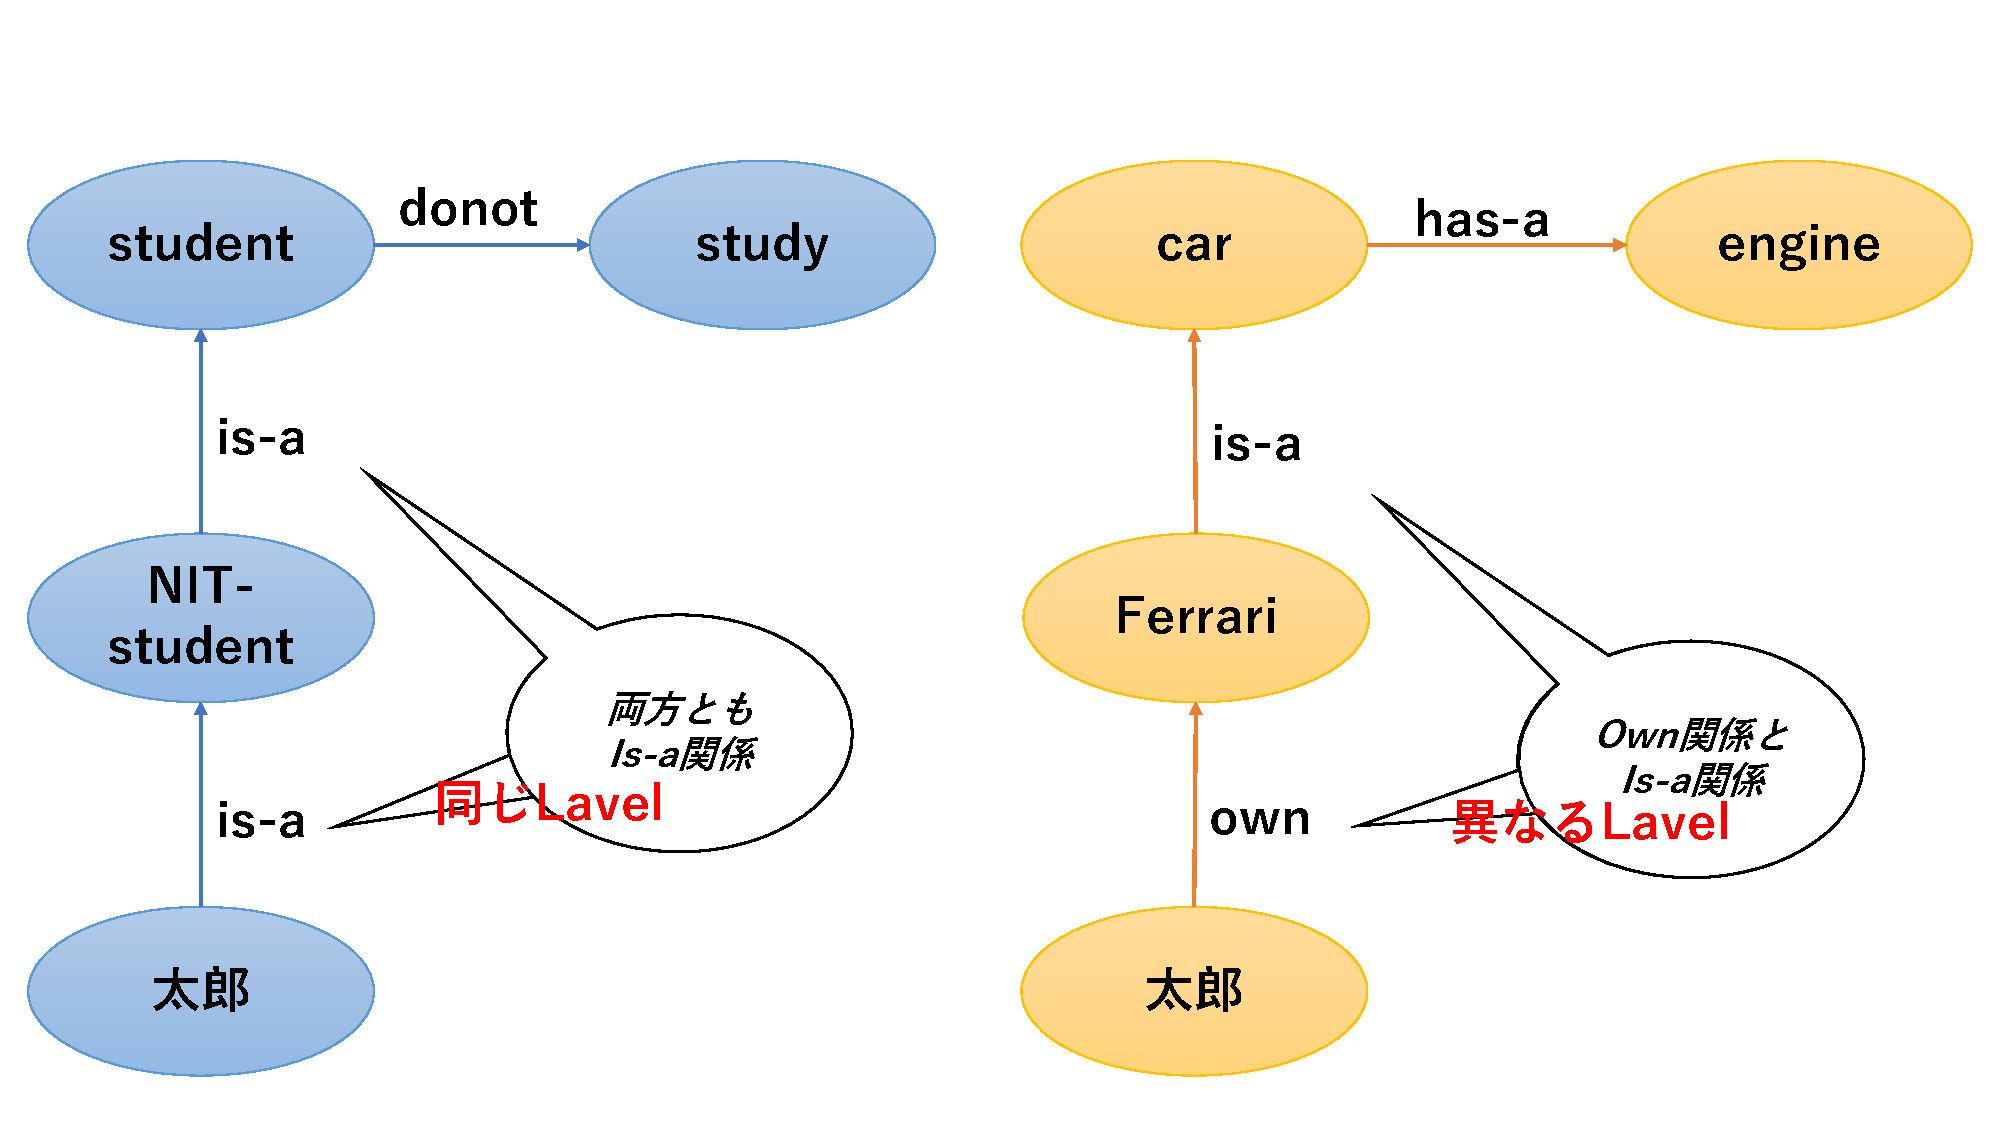
\includegraphics[width = 9cm, pagebox = cropbox, clip]{継承とLabelの対応.pdf}
 \end{center}
 \caption[]{継承とLabelの対応}\label{fig:fig1.1}
\end{figure}

太郎とFerrariのラベル"own"と Ferrariとcarのラベル"is-a"は異なるため, 太郎はcarを持っていることにはならない. 同様に車はエンジンを持つので, つまり太郎はエンジンをもつということは, 文脈上成り立つが, この知識表現ではラベルの違いから成り立たない. その一方で, "太郎は勉強をしない"という文は成り立つ. これは, "is-a"ラベルがNIT-studentもstudentにも成り立ち, 太郎はstudentまでつながれるからである.


\section{感想}
Javaの使い方は, ググってもいいが, 昔しっかり使い込んだ教科書に立ち戻るのも, また一挙である. 今回はScannerクラスとdo-while文の複数入力プログラムをJava入門の教科書から参照した.

英文での質問を処理する際に, 「a」とか「the」とかの前置詞を取るのがめんどくさかった. 私はあまり英語が得意ではないので, Google翻訳先生に頼り, 前置詞を補完, 処理していった. 前置詞は日本人にとってなじみにくい...

%%%%%%%%%%%%%%%%%%%%%%%%%%%%%%%%%%%%%%%%%%%%%%%%%%%%%%%%%%%%%%%%%%%%%%%%%%%%%%
% 参考文献
\begin{thebibliography}{99}
\bibitem{notty} Javaによる知能プログラミング入門 --著:新谷 虎松 \\
\bibitem{notty} 新・明解 Java 入門 --著:柴田望洋 \\
\bibitem{notty} Java 指定型の読み取り --著:Let's プログラミング \\
\url{https://www.javadrive.jp/start/scanner/index2.html}
\bibitem{notty} Google翻訳 --著:Google \\
\url{https://translate.google.com/?hl=ja}
\end{thebibliography}

\end{document}